\chapter{Resultate}
\label{tb-resultate}

Wir konnten die wichtigsten Hauptziele erreichen.
\kort{} erfüllt nun die Grundlage aller wichtigen Anforderungen an eine moderne App.
Nach dem Login wird der Benutzer wie schon bei der \kort{}-\gls{WebApp} zur Kartenansicht weitergeleitet.
Er kann auf einen Marker klicken und gelangt direkt zur Ansicht, um die gewählte Mission zu lösen.
Der Zwischenschritt, dass der Benutzer zuerst gefragt wird, ob er die Lösung kennt, wurde weggelassen.
Somit entfällt ein weiterer Klick, was die Spielmechanik vereinfacht.
Nur noch das Marker-Icon auf der Karte verrät etwas über den Missionstyp und weckt dabei immer noch die Neugier beim Benutzer.

%ToDo: Screenshots

\section{Zielerreichung}

Erreichte Ziele:
\begin{itemize}
	\item Eine \brand{Android}-App mit gleicher Grundfunktionalität, wie die Web-App.
	\item \brand{iOS}-App nur zu Teilen umgesetzt.
	\begin{itemize}
		\item Enthält noch Fehler beim \brand{Google} Sign In
	\end{itemize}
	\item Ein neuer Validierungsmechanismus
	\item Ein Erfahrungsbericht zu \brand{React-Native}.
	\item Die Internationalisierung wurde umgesetzt.
\end{itemize}

\begin{figure}[H]
\subfigure{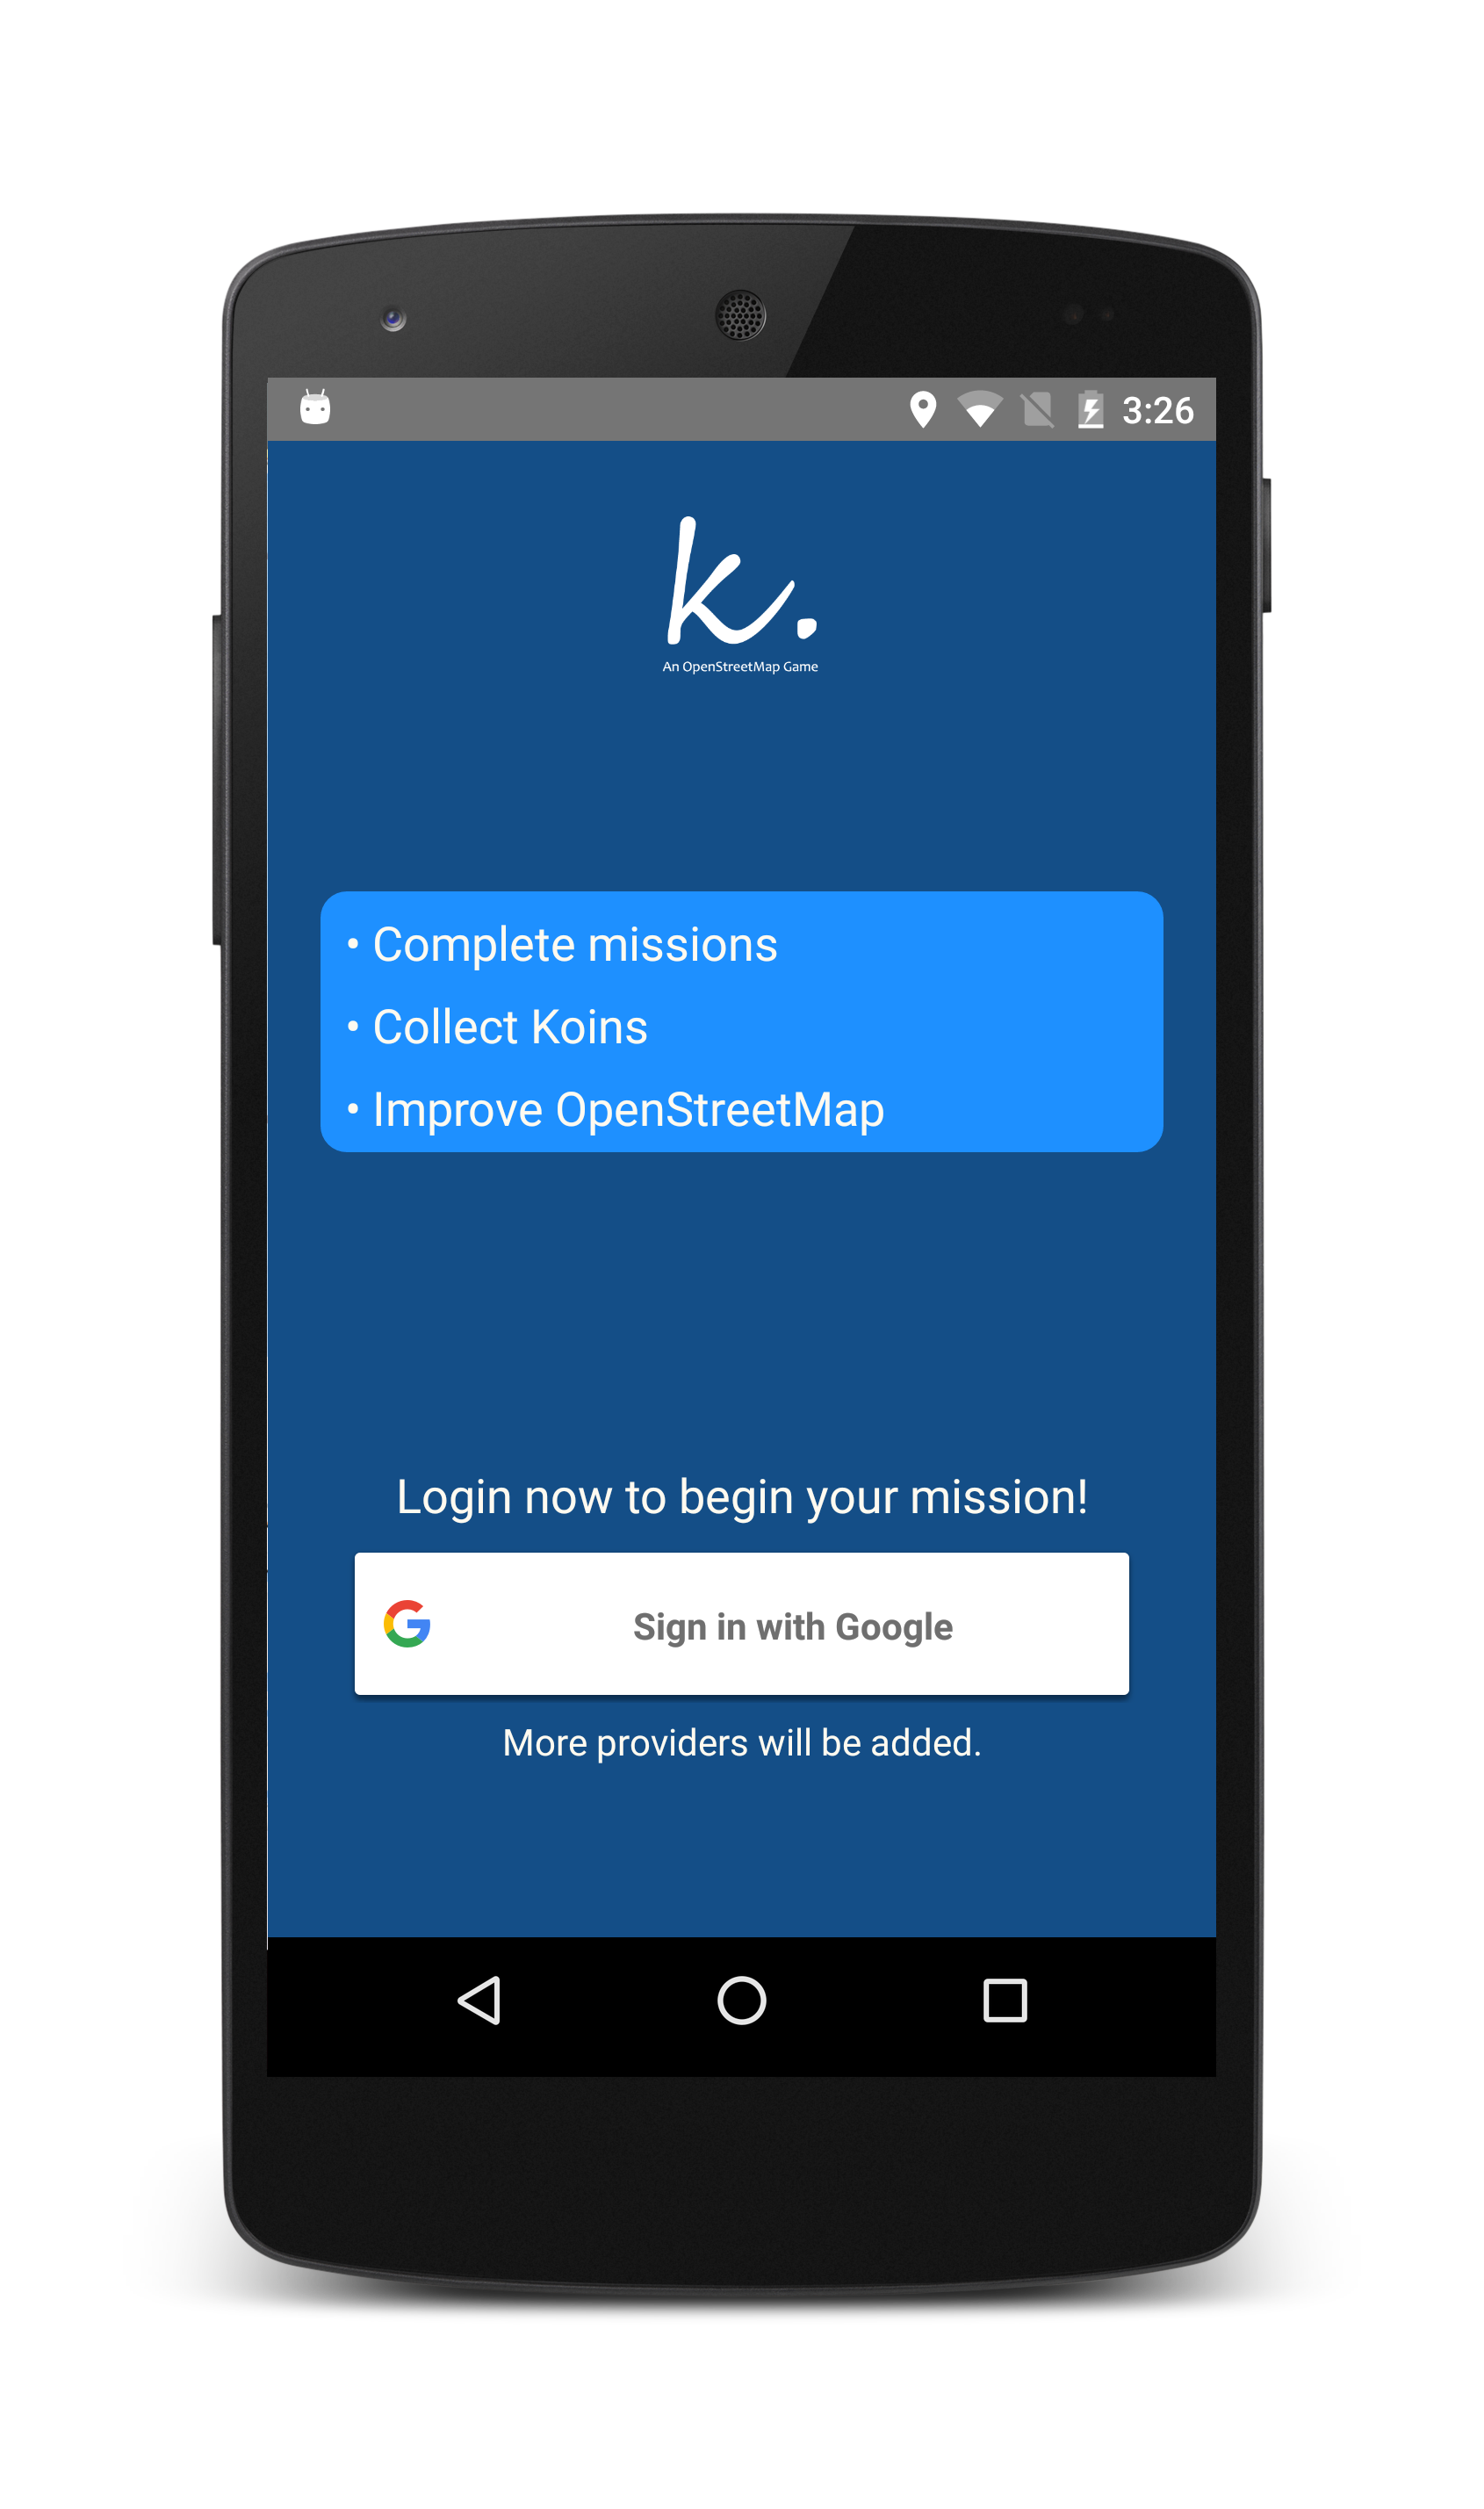
\includegraphics[width=0.3\textwidth]{images/screenshots/login}}
\hfill
\subfigure{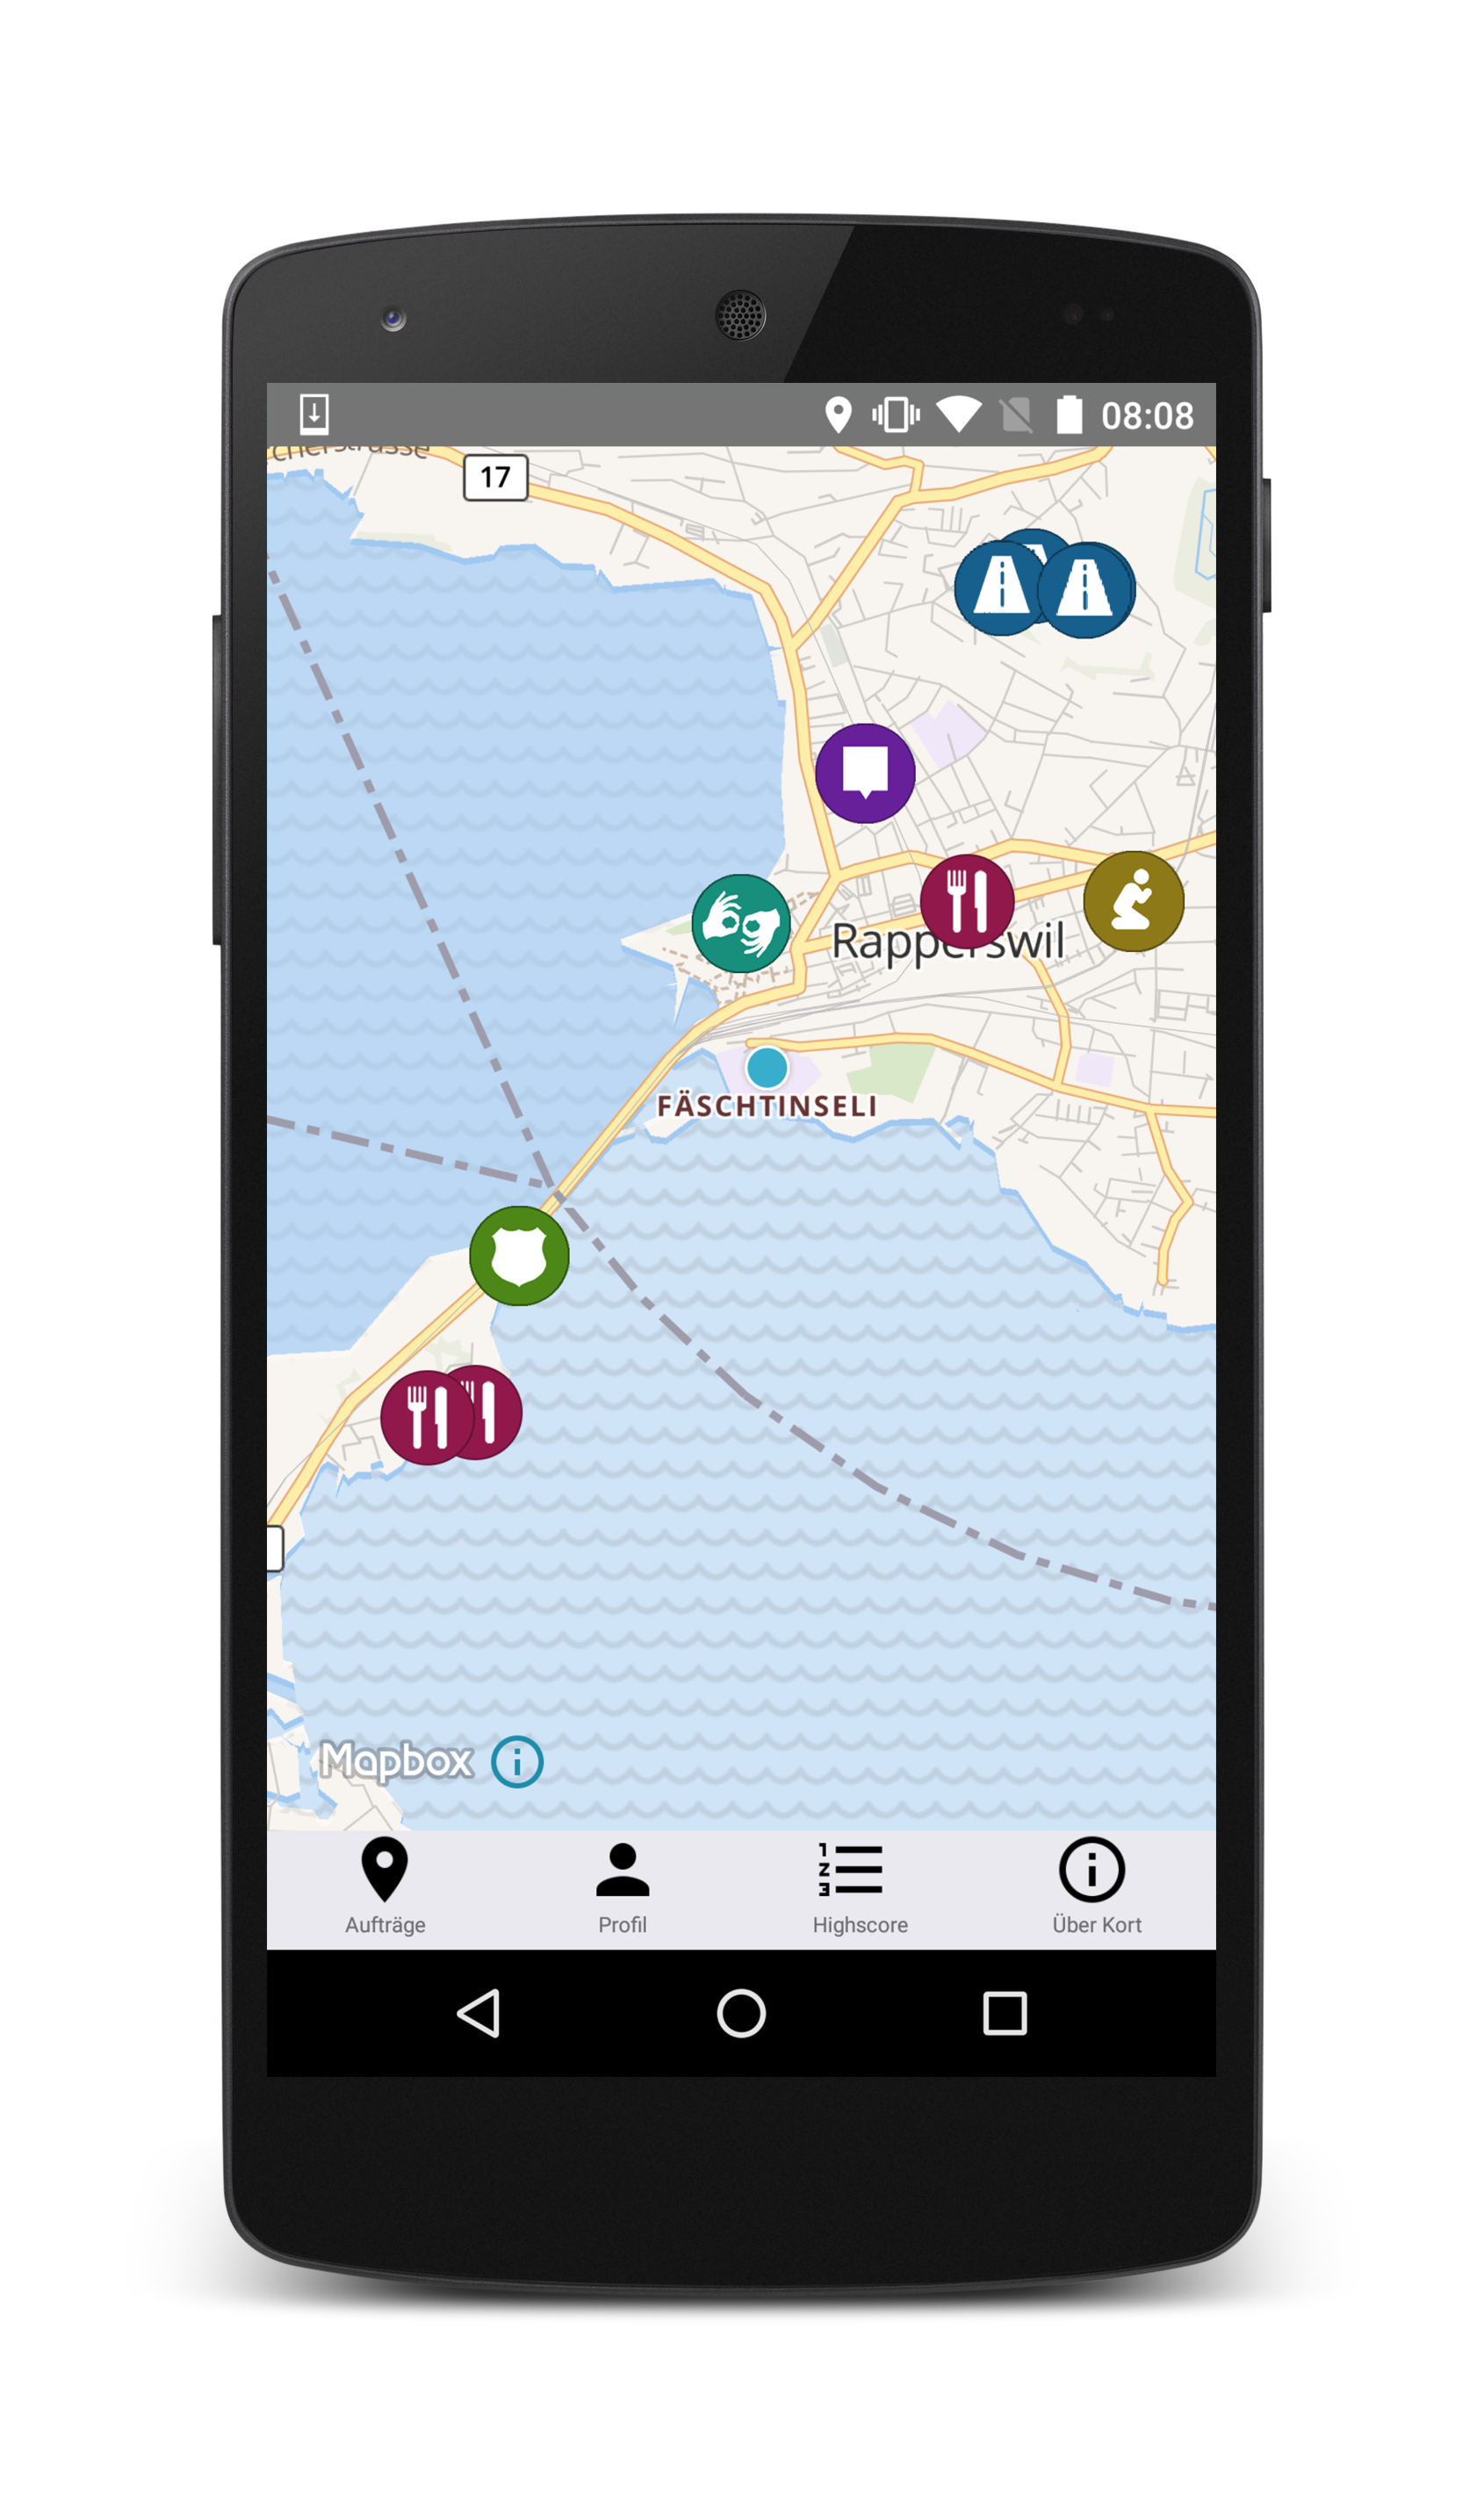
\includegraphics[width=0.3\textwidth]{images/screenshots/missions}}
\hfill
\subfigure{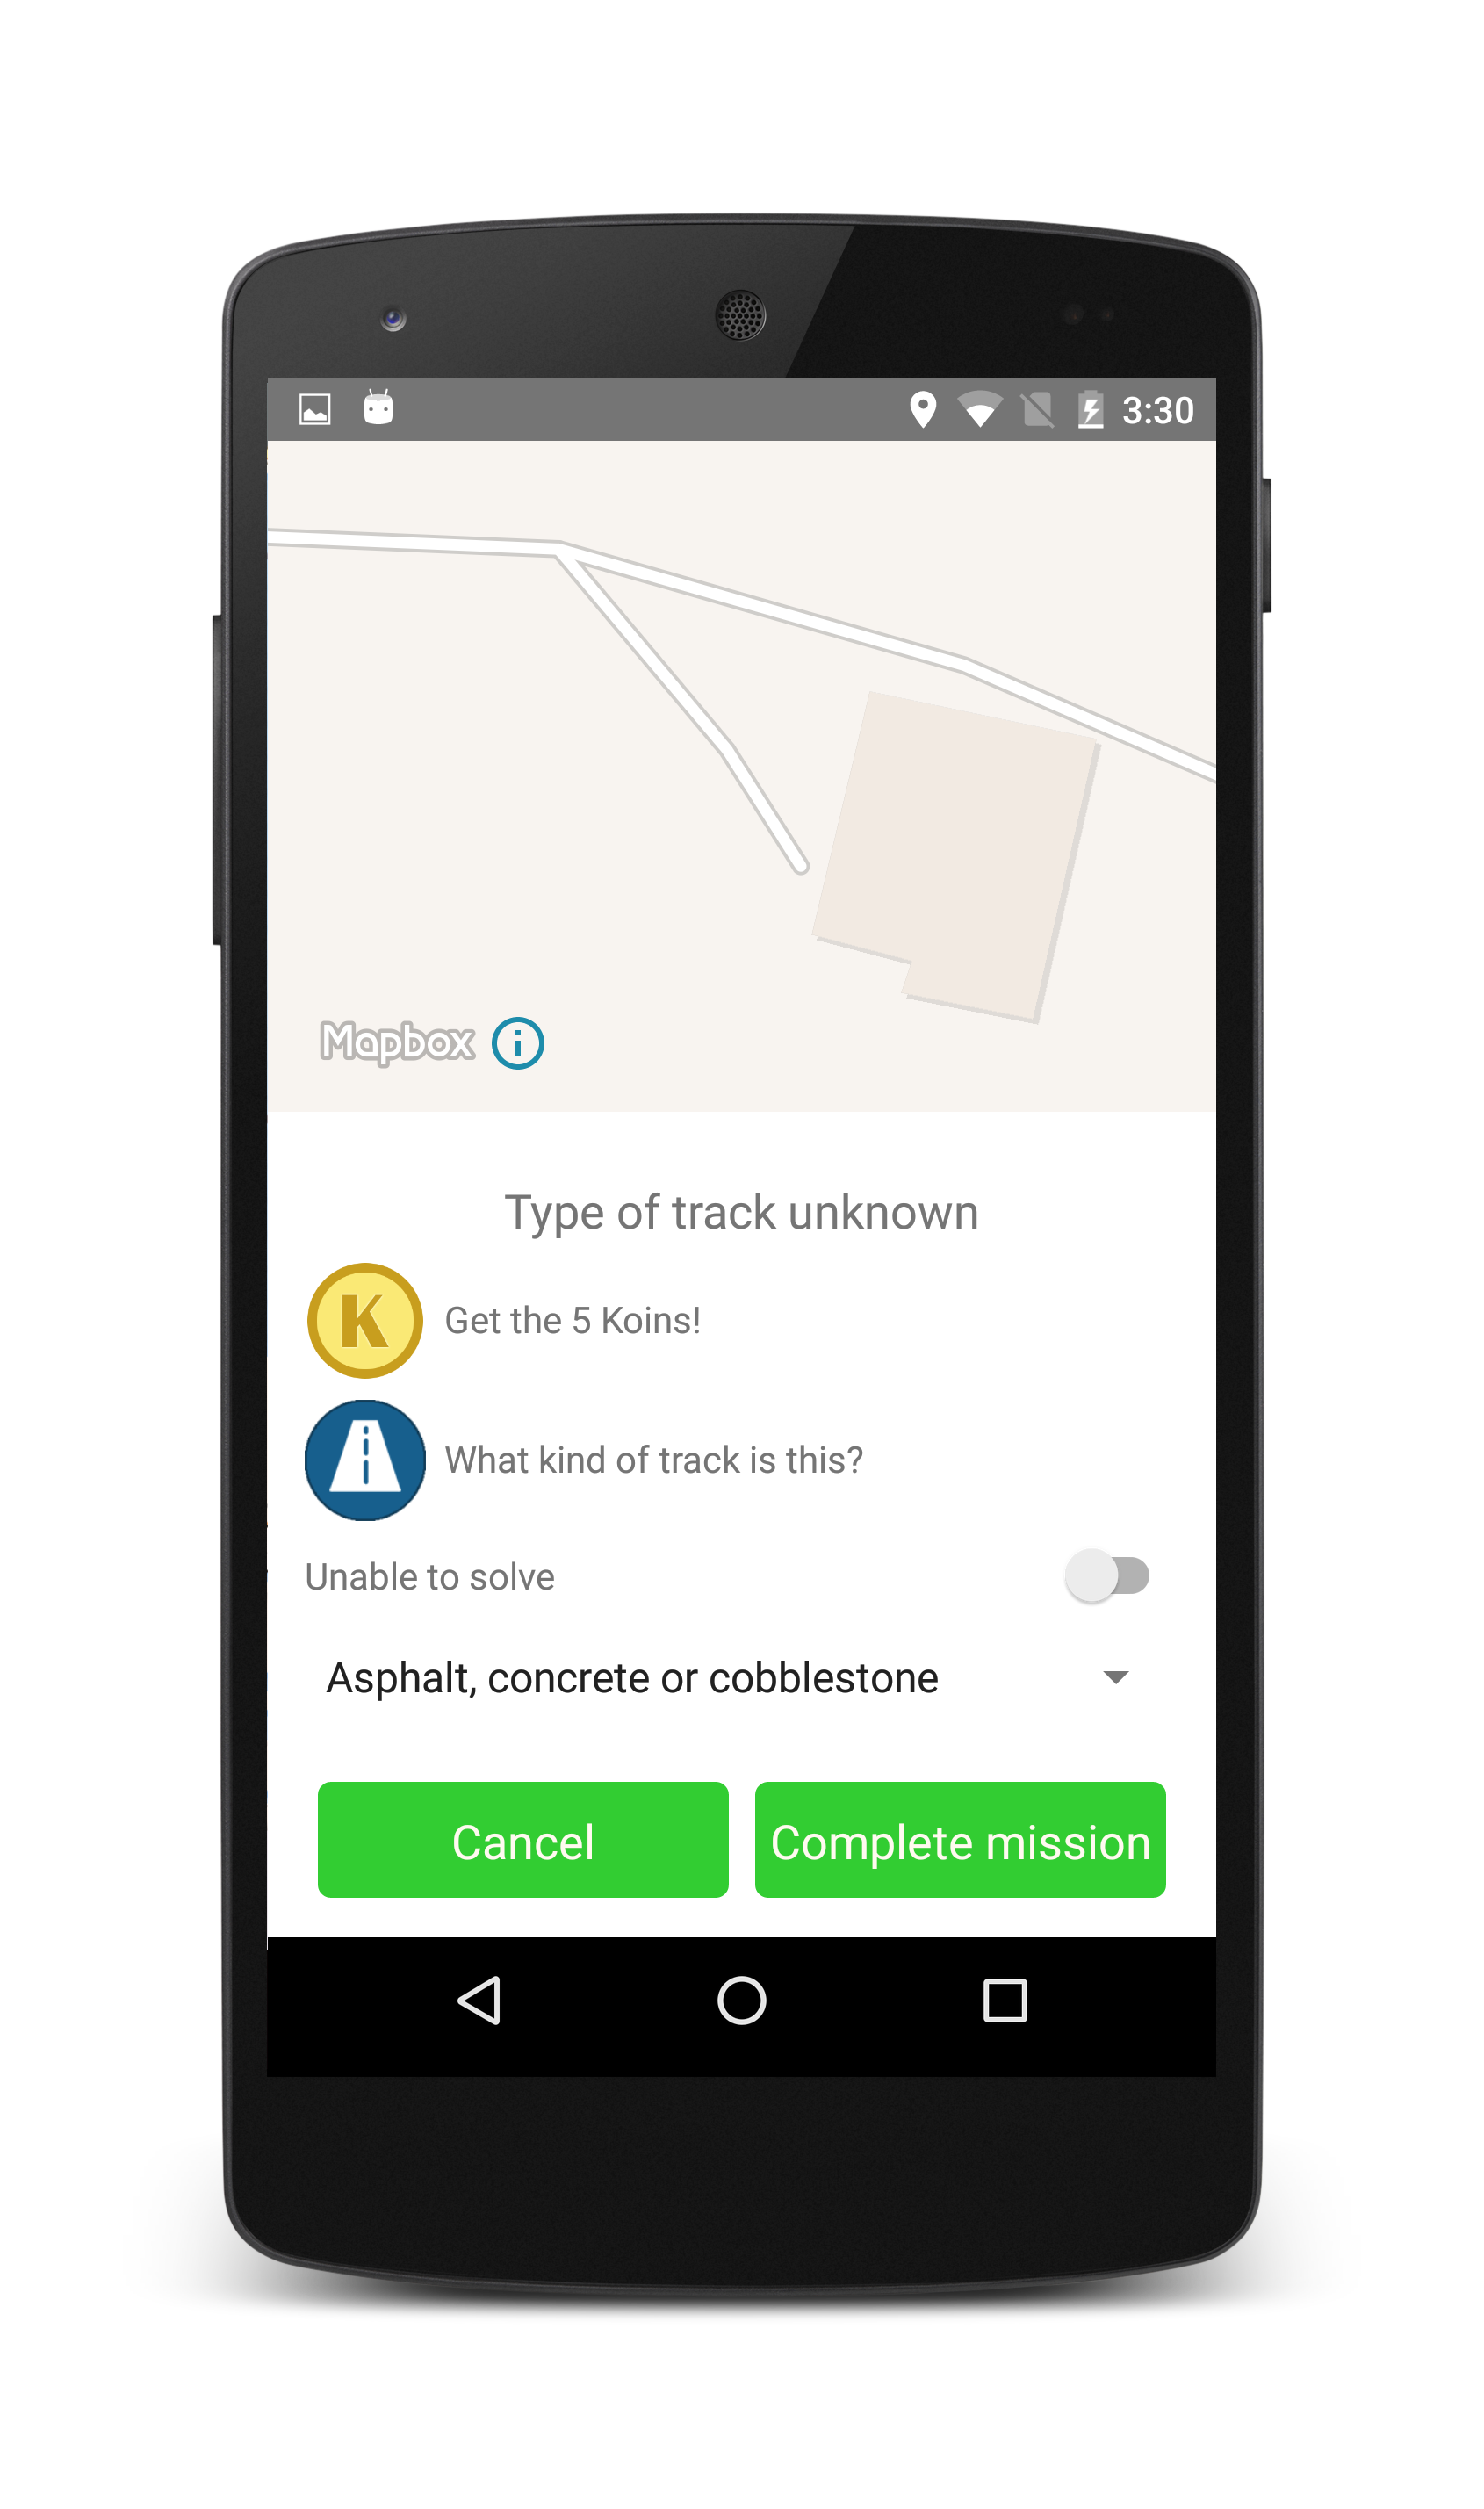
\includegraphics[width=0.3\textwidth]{images/screenshots/solve-mission}}
\caption{\kort{} App}
\label{image-kort-screenshots}
\end{figure}

Das \gls{GUI}-Design ist noch nicht ansprechend und erfüllt nur die minimalen Ansprüche.
Für eine finale Version, die veröffentlicht werden kann, muss das Design aufgebessert werden.

Zu Beginn des Projekts wurde die App für \brand{Android} und \brand{iOS} umgesetzt, wobei die \brand{iOS}-App im späteren Verlauf vernachlässigt werden musste und nicht mehr explizit getestet wurde.
Bei einem kurzen Test gegen Ende des Projekts mussten wir feststellen, dass der \brand{Google} Login nicht funktioniert.

Social-Login wurde nur für \brand{Google} realisiert.

Die Badges, welche vom \gls{Backend} empfangen werden, konnten durch den neuen Validierungsmechanismus nicht mehr verwendet werden.
Das Backend macht nämlich immer noch die Unterscheidung zwischen Missionen und Validierungen.
Die Veröffentlichung im \brand{Google-Play} Store ist im \hyperref[pm-ms9]{Meilenstein 9} aufgeführt, konnte aber leider noch nicht realisiert werden da im Backend noch Probleme beim Erstellen eines neuen Benutzers bestehen.

Wie diese zusätzlichen Arbeiten umgesetzt werden könnten wurde im Kapitel \hyperref[pd-weiterentwicklung-vorgehen]{Vorgehen} dokumentiert.

\section{Ausblick}
Offene Punkte und nächste geplante Arbeiten mit höherer Priorität:

\begin{itemize}
	\item \brand{OSM}-Login
	\item Finale \brand{iOS}- und \brand{Android}-App
	\item Veröffentlichung im \brand{Apple App Store} und \brand{Google Play Store} 
	\item Promotions-Funktion
\end{itemize}

Das genaue Vorgehen, wie die offenen Punkte umgesetzt werden, wird im Kapitel \hyperref[pd-weiterentwicklung-vorgehen]{Vorgehen} beschrieben.
Für die Zukunft gibt es bereits viele weitere Ideen. 
Eine Liste wurde im Kapitel \hyperref[pd-weiterentwicklung-realistisch]{Weiterentwicklung} erstellt. 


\newpage
\section{Persönliche Berichte}
\subsubsection{Dominic Mülhaupt}
Nach dem \hyperref[pm-ms1]{Kickoff Meeting} war ich sehr begeistert von \kort{}.
Der Anfang gestaltete sich dann aber insbesondere in Bezug auf die Planung und die technische Analyse eher harzig.
Ähnlich wie Marino Melchiori hatte ich kaum Kenntnisse in \brand{JavaScript}.
Mit \brand{React} und \brand{React Native} kamen noch zwei weitere grössere Systeme hinzu, womit es am Anfang schwer fiel, zu wissen, wo man überhaupt beginnen soll.
Diesbezüglich bin ich unserem Betreuer, Prof. Stefan Keller, sehr dankbar, dass er uns die nötige Zeit gab, uns in viele der für uns neuen Technologien einzuarbeiten.\newline
Darüber hinaus gab es auch noch mehrere, manchmal kuriose Probleme im Zusammenhang mit dem sich noch immer in Entwicklung befindenden \brand{React Native}.
Dies hat dazu geführt, dass ich oft mehrere Stunden mit Fehlersuche beschäftigt war, was manchmal etwas frustrierend war.
Im späteren Verlauf der Arbeit hat sich aber ein Fluss eingestellt, wobei mich auch die verwendeten Technologien immer mehr überzeugen konnten.
Das Produkt zum Zeitpunkt der \hyperref[pm-ms7]{Abgabe} ist noch nicht vollends befriedigend, da es noch einige Punkte gibt, die sich relativ schnell umsetzen liessen.
Deshalb werde ich auch gerne noch darüber hinaus am Projekt weiterarbeiten.\newline
Ich würde mich freuen, zu einem späteren Zeitpunkt wieder einmal ein Projekt mit \brand{React Native} durchführen zu können, da ich das Konzept sehr ansprechend finde.

\subsubsection{Marino Melchiori}
Beim Start des Projektes hatte ich keine \brand{JavaScript}-Erfahrung. 
Der Einstieg in \brand{JavaScript} war sehr schwer. 
Vor allem das Verstehen des Konzepts von \brand{React} war nochmals etwas ganz Neues. 
Dazu kam Flexbox, das am Anfang für simple Layouts extrem aufwendig und kompliziert wirkte. \newline
Die verwendeten Libraries erzeugten oft unerklärliche Fehler, die nach langem durchforsten von \brand{GitHub}-Issues behoben werden konnten. 
Das verzögerte immer wieder die Planung und unterbrach den Fluss. \newline
Im Verlauf der Arbeit gelang es mir aber, dank der Zusammenarbeit in unserem Team, mich gut  einzuarbeiten.
Das Highlight dieser Arbeit war für mich die Implementation der App mit \brand{React Native} und die Gestaltung der Benutzeroberfläche mit \brand{JSX}. 
Flexbox gefiel mir mit der Zeit immer besser, da die Wiederverwendbarkeit von Layouts sehr praktisch ist. \newline
Trotz all den neuen und teilweise unreifen Technologien ist es uns gelungen, eine gute App-Idee neu zu entwickeln. 
Ich bin froh, dass ich \brand{JavaScript}-Erfahrungen sammeln konnte. 
\brand{React Native} würde ich in Zukunft sehr gerne wieder einsetzen und ich bin überzeugt, dass sich diese Technologie durchsetzen wird. 
